\chapter{Conclusioni}
\label{chap:conc}

Lo scopo di questa tesi era la realizzazione di un prototipo per la domotica d'ufficio che prevedesse l'utilizzo dei beacon.
Al di la della parte pratica di tutto ciò, siamo andati a trattare diverse tecnologie che si stanno sviluppando in questi ultimi anni, sia a livello software che a livello hardware.

Abbiamo visto come il linguaggio JavaScript sia passato da essere utilizzato per l'esecuzione di qualche controllo nelle pagine web tipico degli anni 90, a essere un linguaggio di riferimento per lo sviluppo di applicazioni sia sul front-end che sul back-end.
Infatti, grazie a Node, JavaScript è stato portato anche sui server, diventando un linguaggio universale. 
Per universale intendo la capacità di un programma di essere eseguito su qualsiasi dispositivo indipendentemente dal sistema operativo utilizzato e dall'hardware sottostante.

Abbiamo introdotto l'utilizzo di database documentali al posto di quelli relazionali evidenziandole le principali differenze.
In particolare, grazie all'assenza di una struttura vera e propria, i database documentali sono più adatti in progetti in cui il software viene sviluppato in maniera incrementale.

Con l'introduzione delle WebSocket abbiamo visto una delle tante specifiche introdotte con l'HTML5 che sta rivoluzionando il web.
Grazie a questa, ed altre importanti novità, un programmatore ha tutti gli strumenti necessari per sviluppare un'applicazione da far girare all'interno del proprio browser che ha veramente poco, se non nulla, da invidiare ad una applicazione desktop tradizionale.
   
Per quanto riguarda l'hardware, i beacon sono dispositivi semplici ma allo stesso tempo si possono rivelare molto utili in alcuni contesti come il marketing. 
Al contrario di come molti pensano, i beacon non comunicano informazioni dirette alle app. 
Sono le applicazioni che rilevano la vicinanza di un determinato beacon e una volta identificato eseguono un'azione.
Nel nostro caso specifico, quando uno smartphone con l'app installata rileva di essere entrato nella regione di un beacon invia un comando per pilotare il dispositivo associato.
Nel caso vengano utilizzati per una campagna di marketing, quando uno smartphone rileva un beacon sa di essere nella vicinanze di un determinato negozio, può scaricare dal server le relative promozioni e inviare una notifica all'utente con le offerte più adatte a lui.

    
\section{Il futuro di Proximity System}

Una volta completato il nostro prototipo, con l'aiuto di extrategy e in particolare Silvia Morresi, abbiamo realizzato il modello di business del nostro prodotto.
Per modello di business si intende l'insieme delle soluzioni organizzative e strategiche attraverso le quali l'impresa acquisisce vantaggio competitivo.
Per fare ciò, abbiamo utilizzato uno strumento che utilizza il linguaggio visuale per realizzare modelli di business innovativi: \textbf{Il Business Model Canvas}.
Grazie a questo framework e alla sua efficacia comunicativa tutti possono comprendere elementi complessi che riguardano il funzionamento di un'azienda.

Le descrizioni dettagliate del nostro modello di business e del BMC in generale verranno fatte nella tesi di Marco. 
Per ora, eccovi un'anteprima:
\begin{figure}[htpb!]
  \centering
  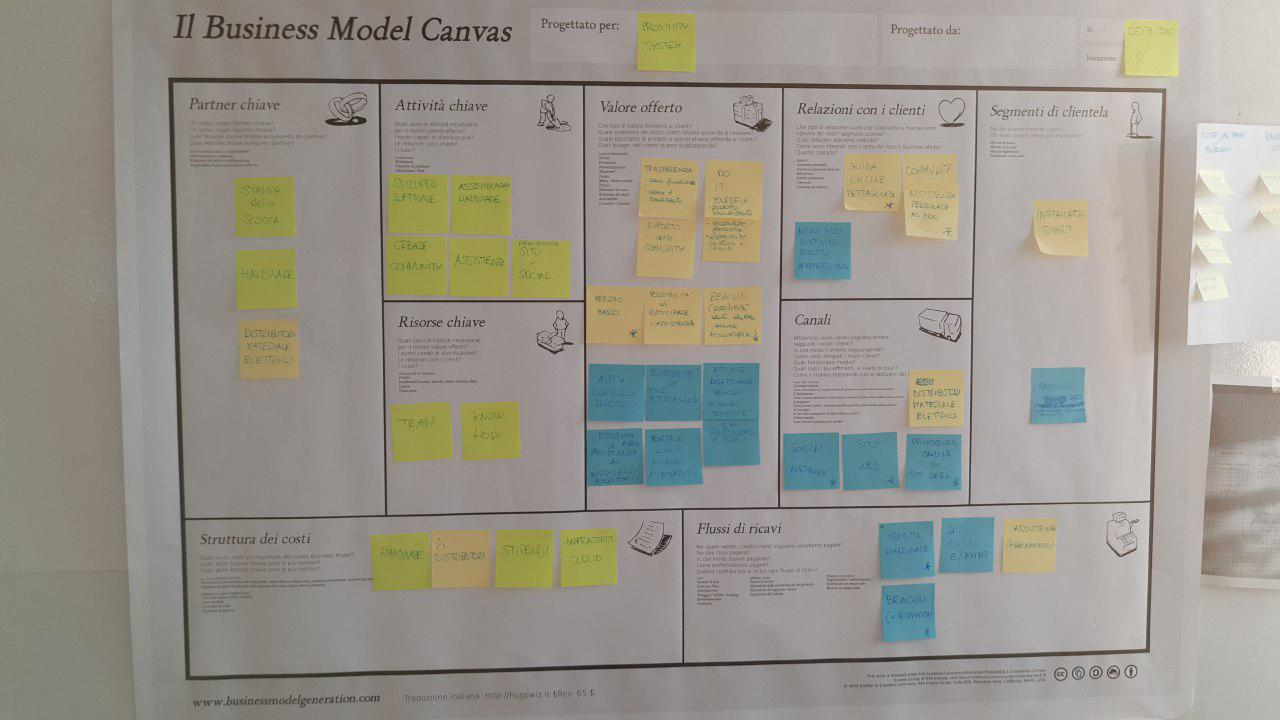
\includegraphics[width=1\textwidth]{bmc}
  \caption{Il nostro Business Model Canvas}
  \label{fig:bmc}
\end{figure}
